\documentclass[12pt]{article}
\usepackage{graphicx}
\usepackage{longtable}
\usepackage[margin=1in]{geometry}
\author{Ryan Young, Eric Rock, John Maloney}
\date{}

\begin{document}

\title{\vspace{50mm} MAESTOR: MAchine and Environment Software Translation Over Ros}
\maketitle
\pagebreak



\tableofcontents
\pagebreak
\section{Introduction}

This repository contains the MAchine and Environment Software Translation Over Ros (MAESTOR) software project. Included are install scripts to generate the execution environment required for MAESTOR, as well as an install script to generate the execution environment for virtualization and visualization of the HUBO robot.\\

MAESTOR was designed to be an easy to use rapid prototyping tool for developing movements on the humanoid robot HUBO. MAESTOR allows you to visualize code in simulation and execute the same code on real hardware. One of the ways that you can create movements on the robot is by making simple to write python scripts that can be powerful enough to create complex movements even walking. MAESTOR is a great development tool for integrating external sensors with HUBO thanks to it using ROS as a communication bus. This user manual will help walk you through using MAESTOR so you can begin to get started on your own scripts and projects.\\ 

\noindent
All examples of commands to run are centred and in italics for example:
\begin{center}
\textit{ls -a}
\end{center}

\section{Software Requirements}
For MAESTOR to run properly you must have all of the following:
\begin{itemize}
	\item Ubuntu 12.04 LTS
	\item ROS Fuerte
	\item OpenRAVE (ROS stack)
	\item hubo-ach
	\item OpenHubo
\end{itemize}

\begin{description}
	\item[Ubuntu 12.04 LTS] \hfill \\
		Ubuntu 12.04 is the operating system that we built MAESTOR for. \\
	\item[ROS Fuerte] \hfill \\
		ROS Fuerte is the Robot Operating System that allows us to communicate using TCP packets to different nodes. MAESTOR is a ROS package and also uses ROS for all of its service communication. \\
		
	\item [OpenRAVE (ROS stack)] \hfill \\
		OpenRAVE is used for visualizing the robot in simulation and also providing the physics in simulation. 
	\item [hubo-ach]\hfill \\
		hubo-ach is how we communicate to the can boards to pass can messages to the motor boards.
	\item [OpenHubo]	\hfill \\
		OpenHubo is an OpenRAVE extension that simulates HUBO specifically. 
\end{description}

\section{Software Overview}
\begin{center}
	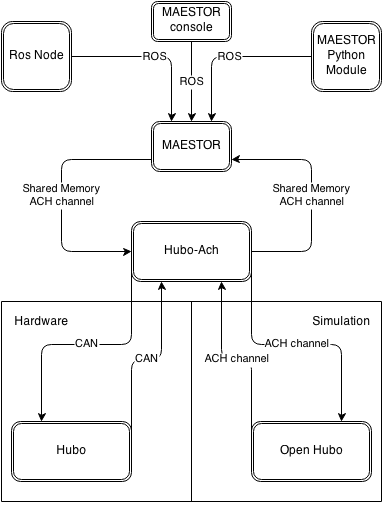
\includegraphics[scale=.75]{Highlevel}
\end{center}

\noindent
MAESTOR is a ROS node that allows advertises ROS services that allows it to interact with other ROS nodes. MAESTOR manipulates the robot of simulation by using the program Hubo-Ach. Hubo-Ach and MAESTOR communicate through shared memory files called ACH channels. Hubo-Ach can operate in either Hardware mode, on a real robot, or in simulation mode using the OpenRAVE extension OpenHubo to simulate Hubo. When operating on hardware Hubo-Ach communicates using the CAN bus on the robot and uses CAN to talk to the motor boards. In simulation Hubo-Ach uses Ach channels to communicate with the simulation. MAESTOR provides access to all of this through ROS and allows more functional joint control with included interpolation functions, inverse kinematics, balancing and more. 

\section{Installation}

Installation scripts exist to install dependencies such as ROS, OpenRAVE, Hubo-Ach and OpenHUBO.

\subsection{Install All packages}
Pay strict attention to permissions for all scripts. Some require root access and some mandate non-root access.\\
\noindent
\\To install all dependencies and complementary packages, change directory to the install directory and run the install all script:
\begin{center}
\textit{./install-all.sh}
\end{center}
\pagebreak
\subsection{Install Packages Independently}

The install all script just calls each of these scripts individually. If there are errors when using the install all script it is recommended to install each package using these install scripts in this order or you can install only the packages you need.  

Installation of ROS:

\begin{center}
	\textit{sudo ./install-ros-fuerte.sh}
\end{center}

Installation of OpenRAVE:
\begin{center}
	\textit{sudo ./install-openrave.sh}
\end{center}

Installation of Hubo-Ach:
\begin{center}
	\textit{	sudo ./install-hubo-ach.sh}
\end{center}
	
Installation of OpenHUBO:
\begin{center}
	\textit{./install-openHubo.sh}
\end{center}

Installation of the MAESTOR ROS pacakge:
\begin{center}
	\textit{./install-maestor.sh}
\end{center}
	
\subsection{Testing Installation}

After installation, it is recommended for the user to interact with these packages in a new terminal in order to ensure that environment variables are properly loaded. If any errors occur, please reboot the operating system and try again,to confirm that the errors are not related to unloaded environment variables.

To test to see if everything is working run the command:

\begin{center}
	\textit{maestor sim-real}
\end{center} 

This will open up the full MAESTOR environment including ROS, OpenHUBO, and hubo-ach. If everything opens up without any errors then your software installed correctly. 
	
\section{Uninstallation}

If you want to remove all traces of MAESTOR and all of it's dependencies from your computer you can do that with the uninstallation script.

Navigate to Maestor-Install-Directory/install/uninstall\\
Run:
\begin{center}
	\textit{	source uninstall.sh}
\end{center}

You will be prompted to uninstall each of the separate components installed by the install scripts. 
NOTE: Using source to call the script is necessary because otherwise it will unable to read the OPENHUBO\_DIR environment variable.
\pagebreak

\section{How to use}

\subsection{Run}

To run MAESTOR, type the command maestor and an argument:

Usage:
\begin{center}
	\textit{maestor $<$Command$>$} 
\end{center}
$<$Command$>$:
	\begin{description}
		\item[sim] \hfill \\
		-Starts MAESTOR with hubo-ach in simulation mode with physics
		\item[sim-real] \hfill \\
		-Start MAESTOR with hubo-ach in simulation mode without physics (Real time)
		\item[real] \hfill \\
		-Starts MAESTOR with hubo-ach in hardware mode
		\item[console] \hfill \\ 
		-Starts the MAESTOR Python console
		\item[kill] \hfill \\
		-Kills MAESTOR, hubo-ach, and roscore
		\item[script $<$scriptName$>$] \hfill \\
		-Runs the python script that is located in the maestor/scripts/ directory with then name $<$scriptName$>$. The script must follow regular python conventions and end with .py as well as be in the correct directory.
	\end{description}

\noindent To actually run MAESTOR you need to choose either the sim, sim-real, or real argument.\\

\noindent The differences between each mode of operation are as follows:
	\begin{description}
		\item[sim] \hfill \\
		-Hubo-Ach runs in simulation mode, and opens the openHubo simulation. Physics is enabled and the positions of motors can be retrieved. Simulation mode with physics enables will run slightly slower than real time. Two terminals will open, one that is running OpenRave and another that is running roscore. The terminal running OpenRave will require elevated privileges. The terminal that you ran MAESTOR from will also require elevated privileges after you give them to OpenRave.
		\item[sim-real] \hfill \\
		-Hubo-Ach runs in simulation mode without physics. This option is meant for previewing intended robot motion, and should be much faster than simulation with physics. You can not retrieve the positions of the motors with physics off. Two terminals will open, one that is running OpenRave and another that is running roscore. The terminal running OpenRave will require elevated privileges. The terminal that you ran MAESTOR from will also require elevated privileges after you give them to OpenRave.
		\item[real] \hfill \\ 
		-Hubo-Ach runs in hardware mode. This option is meant for running MAESTOR on the actual robot. No simulation is opened and a hardware CAN interface is expected. Your terminal will immediately ask for your password then a bunch of text will appear over the password prompt. You can still type your password even though the text is appearing on screen and you need to. 
	\end{description}
	
\noindent When MAESTOR is finished starting up the original terminal that you ran the MAESTOR command from will be back in your control. There are two suggested options for controlling MAESTOR once it is started. The first is opening up the MAESTOR console and the second is using the MAESTOR Python module. Both ways are wrappers that allow you to make service calls over ROS. 

\subsection{The Console}

To open the MAESTOR console type the command in a terminal:
	\begin{center}
		\textit{maestor console}
	\end{center}
Once the console is open you will see a prompt that looks like a regular Python interpreter prompt:

	\begin{center}
		$>>>$
	\end{center}
	
In this prompt you can use any of the MAESTOR functions by typing their names and any arguments they have. To close out of the console you can press ctrl-d when at a blank prompt. You can reopen the console at any time as long as MAESTOR is running. You can find all of the functions that are available for use and their parameters in the table under the functionality section titled MAESTOR Functions. The underlying workings for this console is a Python script that makes direct ROS service calls and returns whatever they return. For more precise work and performing complex movements and tasks it is highly recommended to use the Python module. 

\subsection{Python Module}

To interact with MAESTOR using scripts or your own programs in Python I recommend using the MAESTOR Python module. The MAESTOR Python module is contained in a file called Maestor.py that resides in the maestor/scripts/ directory. I strongly suggest saving scripts in this directory for convenience. If you save your files in a different directory you will either need to add Maestor.py to the PythonPATH or include Maestor.py in the directory that you save your script. 

\subsubsection{Module Functionality}

The MAESTOR Python module is a class that you can import into your Python script or project and create an object of. If you are familiar with ROS the  MAESTOR module creates a ROS node that is used for calling services on the MAESTOR node. If you aren't familiar with ROS you can use the MAESTOR module to avoid having to use it. The MAESTOR module allows you to use all of the functions that are listed in the MAESTOR functions table and a one more that was added for convenience: 

\begin{description}
	\item[waitForJoint($<$Joint$>$)] \hfill \\
	-Blocking call that waits for the joint $<$Joint$>$ to no longer require motion.
\end{description}

\noindent The way that the module works is you create a \textit{maestor} object in your script and call the functions on that object. The object handles all of the ROS stuff and makes the necessary calls. 

\subsubsection{Creating Your Scripts}

To create a script you can run directly, the script must be executable which can be done with the bash command:

\begin{center}
	\textit{chmod +x $<$scriptName$>$}
\end{center}

This command is not a part of MAESTOR but it gives all users on a system the permission to execute that file. For both running scripts directly and running them with the maestor command you need to have the proper shebang. An example of the Python shebang is:

\begin{center}
	\#!usr/bin/env python
\end{center} 

To import the maestor object from the MAESTOR module add this line to your script:

\begin{center}
	\textit{from Maestor import maestor}
\end{center}

This will allow you to create the maestor object. You can create the maestor object by writing something like: 

\begin{center}
	\textit{robot = maestor()}
\end{center}

Where robot is any variable name you want. From there you can make all of the calls by calling the functions on robot as an example:

\begin{center}
	\textit{robot.setProperty("RSP", "position", -1)}
\end{center}

\noindent \textbf{*NOTE*}\\
\noindent Make sure that your script knows where the Maestor.py module file is. This can be done by either adding it to the Python path or having a copy in the directory where your script is. If your script does not know where the Maestor.py module is it will return a lot of error messages.  

Most scripts will require that you run the start up sequence that is described in Section \ref{quickStart}

\subsubsection{Running Your Scripts}


To run scripts that are in the maestor/scripts/ directory you can run the command: 

\begin{center}
	\textit{maestor script $<$scriptName$>$}
\end{center}

Where $<$scriptName$>$ is the name of a script in the directory excluding the .py extension. For example the command:

\begin{center}
	\textit{maestor script testure}
\end{center}

Will run the script testure.py which is located in the maestor/scripts/ directory. An alternative to running your script through the maestor command is to run it directly. 

\begin{center}
	\textit{./$<$scriptName$>$}
\end{center}

Another alternative way of running this is using the Python interpreter in non-interactive mode with the command:

\begin{center}
	\textit{Python $<$scriptName$>$}
\end{center}

If you use the last method of running the scripts then you do not need to include the shebang nor does it have to be executable. Though it is usually good practice to do these things anyway for scripts. 

\subsection{Functionality}

MAESTOR provides different functions through ROS services that can be called through ROS nodes, the MAESTOR console, or using the MAESTOR Python Module. Below is a table of all of the functions that MAESTOR offers and a description of them. 

\begin{center}
	\begin{tabular}{| l | p{8cm}|}
		\hline
		\multicolumn{2}{ | c |}{MAESTOR Functions} \\
		\hline
		\textbf{Function} & \textbf{Description}\\ \hline
		setProperty($<$Joint$>$, $<$Property$>$, $<$Value$>$) 
		& Set the $<$Property$>$ of the $<$Joint$>$ to the $<$Value$>$.  \\ \hline
		loadTrajectory($<$Name$>$, $<$Path$>$, $<$Read$>$) 
		& Load a trajectory into MAESTOR with the name $<$Name$>$ from the $<$Path$>$. The $<$Read$>$ parameter is a boolean  where if it is true the file that is open is read from and if it's false the file is written to in a trajectory format.   \\ \hline
		
		command($<$Name$>$, $<$Target$>$) 
		& Runs the command $<$Name$>$ with the option of $<$Target$>$ where Target is a joint or nothing. The list of all commands is below.  \\ \hline
		
		setProperties($<$Joints$>$, $<$Properties$>$, $<$Values$>$) 
		& Sets multiple properties on multiple joints to different values. $<$Joints$>$, $<$Properties$>$, and $<$Values$>$ each must have the same number of sections that are delimited by white space.  \\ \hline
		
		unignoreFrom($<$Traj$>$, $<$Joint$>$) 
		& Unignore the $<$Joint$>$ column from the trajectory named $<$Traj$>$  \\ \hline
		
		requiresMotion($<$Joint$>$) 
		& Returns True if $<$Joint$>$ is not at its goal position  \\ \hline
		
		getProperties($<$Joint$>$, $<$Properties$>$) 
		& Get the value of specified properties on the joint $<$Joint$>$. $<$Properties$>$ can be a string of properties delimited by spaces.  \\ \hline
		
		ignoreAllFrom($<$Traj$>$) 
		& Ignore all of the joint columns in the trajectory named $<$Traj$>$  \\ \hline
		
		initRobot($<$Path$>$) 
		& Initialize the robot with the init file specified by $<$Path$>$. The empty string "" denotes the default path. Do not run this function more than once in a session.  \\ \hline
		
		startTrajectory($<$Traj$>$) 
		& Starts the trajectory with the name $<$Traj$>$  \\ \hline
		
		ignoreFrom($<$Traj$>$, $<$Joint$>$) 
		& Ignore the $<$Joint$>$ column from the trajectory named $<$Traj$>$  \\ \hline
		
		setTrigger($<$Traj$>$, $<$Frame$>$, $<$TargetTraj$>$)
		& Sets a trigger at the $<$Frame$>$ in $<$Traj$>$ to stop executing $<$Traj$>$ and begin executing $<$TargetTraj$>$  \\ \hline
		
		unignoreAllFrom($<$Traj$>$)
		& Unignore all of the joint columns in the trajectory named $<$Traj$>$   \\ \hline
		
		extendTrajectory($<$Traj$>$, $<$Path$>$)
		& Appends the trajectory located at $<$Path$>$ to the end of the loaded trajectory $<$Traj$>$  \\ \hline
		
		stopTrajectory($<$Traj$>$)
		& Stops executing the trajectory $<$Traj$>$  \\ \hline
	
	\end{tabular}
\end{center}

\pagebreak 

\subsubsection{Commands}

A lot of how MAESTOR operates is through the use of commands and setting and getting properties. This section will talk about all of the different commands that can be run using the command function and all of the properties that you can get and set on joints.\\

MAESTOR commands can be run using the function: 

\begin{center}
	\textit{command($<$Command$>$, $<$Target$>$)}
\end{center}

Where $<$Command$>$ can be a number of different commands where some have a target and others do not. The Table below goes through all of the commands and if it has a target parameter what it is. Both $<$Command$>$ and $<$Target$>$ must be strings so if the target is empty the empty string must be passed, e.g.

\begin{center}
	\textit{command("HomeAll", "")}
\end{center}

\begin{center}
	\begin{tabular}{| l | l | p{8cm}|}
	\hline 
	\multicolumn{3}{ | c |}{Commands}\\ \hline
	\textbf{Command} & \textbf{Target} & \textbf{Description}\\ \hline
	
	Enable & $<$Joint$>$ & Enables the joint named $<$Joint$>$\\ \hline
	
	EnableAll & & Enables all of the joints on the robot\\ \hline
	
	Disable & $<$Joint$>$ & Disables the joint named $<$Joint$>$\\ \hline
	
	DisableAll & & Disables all of the joints on the robot\\ \hline
	
	ResetJoint & $<$Joint$>$ & Reset the board of the joint named $<$Joint$>$\\ \hline
	
	ResetAll & & Reset all of the boards on the robot\\ \hline
	
	Home & $<$Joint$>$ & Home the joint named $<$Joint$>$\\ \hline
	
	HomeAll & & Home all of the joints on the robot\\ \hline
	
	InitializeSensors & & Initialize the sensors on the robot to begin receiving feedback from them\\ \hline
	
	Zero & $<$Joint$>$ & Return the $<$Joint$>$'s position to zero\\ \hline
	
	ZeroAll & & Return all of the joint's positions to zero\\ \hline
	
	BalanceOn & & Turn active balancing on\\ \hline
	
	BalanceOff & & Turn active balancing off\\ \hline
	
	\end{tabular}
\end{center}

\subsubsection{Properties}
For the functions getProperties, setProperty, and setProperties MAESTOR either sets or get properties on robot components. For each of the commands the syntax is slightly different.
\begin{description}
	\item[setProperty($<$Joint$>$, $<$Property$>$, $<$Value$>$)] \hfill \\
	-This function takes a string $<$Joint$>$ which can be any robot component and sets the property specified by a string $<$Property$>$ to the value $<$Value$>$ where $<$Value$>$ is a float. An example is:
	
	\begin{center}
		\textit{setProperty("RSP", "position", -1)}
	\end{center}
	
	\item[setProperties($<$Joints$>$, $<$Properties$>$, $<$Values$>$)] \hfill \\
	-This function takes strings of robots components, properties, and values each set must be delimited by spaces. The string of robot components is passed in as $<$Joints$>$, string of properties as $<$Properties$>$ and the string of values as $<$Values$>$. An example is:
	
	\begin{center}
		\textit{setProperty("RSP", "position", -1)}
	\end{center}
	
	\item[getProperties($<$Joint$>$, $<$Properties$>$)] \hfill \\
	-This function takes in a robot component as a string for $<$Joint$>$ and a space delimited list of properties for $<$Properties$>$. An example is:
	
	\begin{center}
		\textit{getProperties("RSP", "position velocity goal")}
	\end{center}
	
\end{description}


\noindent Not every component has every type of property but below is a table of all of the properties in MAESTOR and the components that have those properties. 

\begin{center}
	\begin{longtable}{| l | l | p{7cm} |}
		\hline 
		\multicolumn{3}{ | c |}{Properties}\\ \hline
		\textbf{Property} & \textbf{Components} & \textbf{Description}\\ \hline
		
		position & Joints, Meta Joints & The current encoder read position of the joint\\ \hline
		
		goal & Joints, Meta Joints & The current goal position of the joint\\ \hline
		
		speed & Joints, Meta Joints & The current set speed for interpolation\\ \hline
		
		inter\_step & Joints, Meta Joints & The current interpolation step.\textbf{*** *WARNING*} \\ \hline
		
		velocity & Joints, Meta Joints & The current moving speed of the joint as read from the encoder \\ \hline
		
		goal\_time & Joints, Meta Joints & The time it is estimated to finish interpolating \\ \hline
		
		motion\_type & Joints & The type of motion that the joint should use. \\ \hline
		
		temp & Joints & The temperature of the joint \\ \hline
		
		homed & Joints & A boolean that signals if the joint is homed \\ \hline
		
		zeroed & Joints & A boolean that signals if the joint is zeroed \\ \hline
		
		errored & Joints & A boolean that tells if a joint has an error \\ \hline
		
		jamError & Joints & A boolean that tells if a joint has a jam error \\ \hline
		
		PWMSaturatedError & Joints & A boolean that tells if a joint has a saturation error \\ \hline
		
		bigError & Joints & A boolean that tells if a joint has a big error \\ \hline
		
		encoderError & Joints & A boolean that tells if a joint has a encoder error \\ \hline
		
		driveFaultError & Joints & A boolean that tells if a joint has a drive error \\ \hline
		
		posMinError & Joints & A boolean that tells if a joint has a position minimum error \\ \hline
		
		posMaxError & Joints & A boolean that tells if a joint has a position maximum error \\ \hline
		
		velocityError & Joints & A boolean that tells if a joint has a velocity error \\ \hline
		
		accelerationError & Joints & A boolean that tells if a joint has a acceleration error \\ \hline
		
		tempError & Joints & A boolean that tells if a joint has a temperature error \\ \hline
		
		x\_acc & IMU & The acceleration in the X direction \\ \hline
		
		y\_acc & IMU & The acceleration in the Y direction \\ \hline
		
		z\_acc & IMU & The acceleration in the Z direction \\ \hline
		
		x\_rot & IMU & The rotation about the X axis\\ \hline
		
		y\_rot & IMU & The rotation about the Y axis\\ \hline
		
		m\_x & FT & The moment in the X direction \\ \hline
		
		m\_y & FT & The moment in the Y direction \\ \hline
		
		f\_z & FT & The force in the Z direction \\ \hline
		
		meta\_value & Meta Joint & The forward kinematics position of the meta joint. Getting the position of the meta joint returns a more accurate version of this. \\ \hline
		
		
	\end{longtable}
\end{center}

\textbf{*** WARNING:} Manipulating the interpolation step in any way may cause the robot to skip an interpolation step. The interpolation step is generated using a fourth order polynomial whose coefficients are calculated when the position is set. Manipulating an interpolation step could cause serious harm to the robot because that is the number that is sent to the motor boards. If it is required to manipulate the interpolation use extreme caution in operation. 

\subsection{Initialization}

Before you move the robot joints it is very important that you initialize the robot. This includes initializing the software, homing all of the joints, enabling the joints, and initializing the sensors. The following section will walk you through how to do this.\\

The first thing to do is to initialize the software this is done with the command:
	\begin{center}
		\textit{initRobot($<$Path$>$)}
	\end{center}

Where path is a string and the empty string, "", refers to the default directory. The default directory is:
 
\begin{center}
	/opt/ros/fuerte/stacks/maestor/models/hubo\_default.xml
\end{center}

This command loads Robot configuration information from the xml file specified. 
Before this command, MAESTOR cannot perform any other commands or functions.\\

The next thing you have to do is home the joints. Homing is when the joints move to their default zero position, their home. This step is not required when running any type of simulation and if it is done in simulation you will not see any movement. When you run HomeAll you can not move any joints for about 10 seconds so be careful about this when homing in simulation. You can home all of the joints by running the command:

	\begin{center}
		\textit{command("HomeAll", "")}
	\end{center}

If you want to home a single joint instead of all of the joints you can use the command:

	\begin{center}
		\textit{command("Home", $<$JointName$>$)}
	\end{center}
	
\noindent \textbf{*NOTE*} It is best to home the joints multiple times until every joint is in the correct home position. Occasionally some joints may get stuck in strange positions especially the wrists. In these cases you can reset the joint using the command:

	\begin{center}
		\textit{command("ResetJoint", $<$JointName$>$)}
	\end{center}

Once you have all of the joints homed correctly it's time to enable them for control. Before you do this step make sure that every joint is in the correct home position. If it is off from it the joint will jump to the 0 position as soon as you enable. This can be very hazardous and potentially draw to much current on the real robot. In simulation you can enable right after you initialize MAESTOR. To enable the joints run the command:

	\begin{center}
		\textit{command("EnableAll", "")}
	\end{center}
	
From here you are fully initialized and are ready to control the robot. I recommend running these initialization methods by hand in the MAESTOR console then running scripts for motions. The reason I say this is because when you run everything on the real robot it may take a large number of homing attempts before you get it right. 

\subsection{Meta Joints}

MAESTOR handles its implementation of inverse kinematics by using an abstraction that we call Meta Joints. Meta Joints are special robot components then control a group of regular joints. For example the Right Foot Meta Joints manipulate all of the joints in the right leg. MAESTOR has implementation for Forward and Inverse Kinematics for the legs and a simplified Forward and Inverse Kinematics for the arms. Both implementations of the Inverse kinematics are done using geometry not inverse solvers so they are reasonably quick. 

\begin{description}
	\item[Foot Meta Joints]
	-Each foot has three meta joints. They are the RFX, RFY, and RFZ and the LFX, LFY, and LFZ. The X an Y coordinates of both feet start at zero and the Z coordinates start at -.56 units. To crouch down you can run the command: 
	\begin{center}
		\textit{setProperties("RFZ LFZ", "position position", "-.52 -.52")}
	\end{center}
	
	
	\item[Arm Meta Joints]
	-Each arm has three meta joints. They are the RAX, RAY, and RAZ and the LAX, LAY, and LAZ. There aren't any default values for the Arm meta joints but it may take some playing around in simulation to get used to where the best values for the meta joints are. 
	
	\item[Neck Meta Joints]
	-The neck originally does not have a neck pitch and neck roll on the hubo2+ so we created meta joints that work like a neck pitch and neck roll. They are NKP and NKR. 
	
\end{description}
Each three letter code above is a Meta Joint and have properties that can be set and got.
\subsection{Moving}

One of the biggest things that you will want to do with MAESTOR is move joints. This can be done with the setProperty function.\\ 

To move A Single Joint:
	\begin{center}
		\textit{setProperty($<$Joint$>$, "position", $<$value$>$)}
	\end{center}
	
A grounded example of this command could be:
	\begin{center}
		\textit{setProperty("RSP", "position", -1)}
	\end{center}

When you set the position of a joint to a value MAESTOR moves the joints at the current speed that it is set at to that position. The value should be in radians. A good check for safe positions for HUBO is to use Hubo-in-the-browser written by William Hilton. 

To change the speed that the joint moves you can use the command:
	\begin{center}
		\textit{setProperty($<$Joint$>$, "speed", $<$value$>$)}
	\end{center}
	
The speed is in radians per second and should only be a positive number. You can use decimals for speeds such as .3 and 1.5 as well as whole number values. I do not recommend using speeds faster than 2 but there is no coded upper limit. 


\subsubsection{Joint Motion types}

These are motion types that come from hubo-ach for each joint. The default is 1 and I highly recommend not changing it to anything else. But the option is there.  

0 - Filtered motion. Hubo-ach will internally filter and interpolate the goal position.

1 - Non-filtered motion. Hubo-ach will set the motor reference directly.

	
\subsection{Feedback}

Another important feature that Maestor has is feedback. All of the feed back can be done with the getProperties function. I do not recommend trying to implement time critical feedback loops using the getProperties function because of ROS latency issues. If you really really really want to implement time critical feed back email Ryan Young: rdy29@drexel.edu and he can help you to do it.  

To request multiple values from a single joint use the command:
    \begin{center}
		\textit{getProperties($<$Joint$>$, $<$Properties$>$)}
	\end{center}

Where properties is a space delimited string list of properties or a single property. The list of properties can be found in Table 3


\subsection{Running Trajectories}

\begin{center}
\textbf{***WARNING***}
\end{center}
Trajectories can be very dangerous. There is no interpolation of the joint angles that you put in your trajectory file. If the gap is too big or the trajectory file has a bug in it the robot may cause harm to its self. Use trajectories with caution.\\

A trajectory is defined as a chain of non-zero length of Whitespace Separated Value files. Each file may contain columns of position values to be sent sequentially to joints which may be indicated by an optional header. A default header assumes that all 40 joints will be included in the following order:

\begin{center}
RHY RHR RHP RKP RAP RAR LHY LHR LHP LKP LAP LAR RSP RSR RSY REP RWY RWR RWP LSP LSR LSY LEP LWY LWR LWP NKY NK1 NK2 WST RF1 RF2 RF3 RF4 RF5 LF1 LF2 LF3 LF4 LF5
\end{center}

All trajectory commands take strings as arguments unless specified otherwise. To load a trajectory, the following command is used:

    \begin{center}
		\textit{loadTrajectory($<$Trajectory Name$>$, $<$path to trajectory$>$, $<$playback$>$)}
	\end{center}

Where Trajectory Name is a short name to be used to refer to that trajectory later, and playback is a boolean value that should be passed as true if the trajectory is to be read from and false if the trajectory is to be written to.\\
       
To run a trajectory that is loaded:
    \begin{center}
		\textit{startTrajectory($<$Trajectory Name$>$)}
	\end{center}
    
To stop a running trajectory:
	\begin{center}
		\textit{stopTrajectory($<$Trajectory Name$>$)}
	\end{center}
    


In addition, Trajectories have the following useful features:\\

To force a trajectory to ignore an input from one of its named columns, use this command:
    \begin{center}
    	\textit{ignoreFrom($<$Trajectory Name$>$, $<$Column Name$>$)}
    \end{center}

To unignore a previously ignored column:
    \begin{center}
    	\textit{unignoreFrom($<$Trajectory Name$>$, $<$Column Name$>$)}
    \end{center}

To ignore all columns:
    \begin{center}
    	\textit{ignoreAllFrom($<$Trajectory Name$>$)}
	\end{center}

To unignore all columns: 
    \begin{center}
    	\textit{unignoreAllFrom($<$Trajectory Name$>$)}
	\end{center}

To append a trajectory file to the end of a loaded trajectory*:
    \begin{center}
    	\textit{extendTrajectory($<$Trajectory Name$>$, $<$path to trajectory$>$)}
    \end{center}

\noindent * A trajectory may only be extended if the new trajectory has the same number of columns, the same columns present (not 
necessarily in the same order), and must start relatively close to the last position vector of the current trajectory.
Ignoring extra columns from loaded trajectories may be used to extend trajectories with shorter columns.\\

\noindent To set a trigger for another loaded trajectory** to be played at a certain integer frame***:
    \begin{center}
    	\textit{setFrame($<$Trajectory Name$>$, $<$frame number$>$, $<$Trajectory Name to be Loaded$>$)}
    \end{center}

\noindent ** This method can be used to have a trajectory start itself when the trajectory has finished\\

\noindent *** The "frame" of the trajectory is the number of rows of data which have been read. Comments/headers/empty lines do not count.
A user can specify a frame of -1 to load another trajectory at the end of the given trajectory.

\subsection{Stopping}

Once MAESTOR is started it will run continuously in the back ground as will all of it's dependant packages. To stop MAESTOR run this command in a bash terminal:
	\begin{center}
		\textit{maestor kill}
	\end{center}

	
\section{Quick Start} \label{quickStart}

If you want to get started immediately and read about the details of what you can do later, follow these steps:

	- Run the MAESTOR run script: 
			\begin{center}
				\textit{maestor (run type)}
			\end{center}
		For example, if running in simulation:
            \begin{center}
				\textit{maestor sim}
		    \end{center}
        or, on hardware:
            \begin{center}
				\textit{maestor real}
			\end{center}
		
\noindent If you chose "real" as your run type:
	
		- A terminal should have opened on tty7 (This may be different if there are already processes running on these terminals.)
		
		- It is not required but it is highly recommended to open tty7 (Ctrl - Alt - F7) and make sure the hubo-ach console is running (It may require elevated privileges.)\\

\noindent If you chose "sim" as your run type:
		
		- X Terminals should have opened with hubo ach, roscore and additional simulation windows. Hubo-Ach's terminal will require elevated privileges. Type your password to give them. 
		
		-On occasion one of the xterminals will be directly over top of the other. If this happens and the one running hubo-ach that needs elevated permissions is on the bottom, simply move the top one and give hubo-ach permission. \\
		
\noindent Once everything has finished starting up for both real and simulation, the terminal you started MAESTOR in will be back in your control. 
	
\noindent To open the MAESTOR console type the command:
		\begin{center}
			\textit{maestor console}
		\end{center}

This will give you a python console that has the MAESTOR api and commands loaded. The function ls() will give you a list of all the functions you have available. Each console line starts with: $>>>$ like the Python Interpreter. 

	-To begin controlling the robot or the simulation you must first initialize the robot:
		
		\begin{center}
			\textit{initRobot("")}
		\end{center}          
		
		The parameter is the path to a config file. Empty string is default

	- Next the joints must be homed. This is especially important in hardware mode. Usually when operating HUBO you will have to reset joints and re-home a few times before you can enable the robot. You can home using the command:
		
		\begin{center}
			\textit{command("HomeAll", "")}
		\end{center}

    - In order to move the joints they must be enabled. This can be done with the command EnableAll
		\begin{center}
			\textit{command("EnableAll", "")}
		\end{center}
		

			
	- From here the robot in hardware or simulation can move all of its joints. A simple test is to move the right arm up 
		\begin{center}
			\textit{setProperty("RSP", "position", -1)}
		\end{center}
		 
		
\noindent 
The robot should move its arm up. From here you can begin to manipulate joints from the console using the setProperty function. A detailed guide listing the functionality is below in the How to use section.
	
\section{External Sensors and Demos}
	Because MAESTOR is built off of ROS services it can be used to integrate external sensors with controlling HUBO. A lot of the demos that we have made use this feature and I suggest taking a look at them if you want to get an idea of how it works. It usually consists of creating your own Python scripts with a maestor object and another object that handles the external sensors. \\

To run hubo demos with MAESTOR, download them from the github repositories: 

	\begin{flushleft}
		https://github.com/RyanYoung25/FaceTrackingWaistDemo
		https://github.com/RyanYoung25/TwoArmSoundDemo
		https://github.com/RyanYoung25/BiotacArmDemo
	\end{flushleft}


Each demo has a README with installation instructions which includes specifying them in the ros package path. \\

Some demos require other dependencies, see their README for more information. 

\section{Extras}

\subsection{Default Joint Name scheme}

Joints:\\

\noindent WST		Waist\\
NKY		Neck Yaw\\
NK1		Neck Tilt 1\\
NK2		Neck Tilt 2\\
LSP		Left Shoulder Pitch\\
LSR		Left Shoulder Roll\\
LSY		Left Shoulder Yaw\\
LEP		Left Elbow Pitch\\
LWY		Left Wrist Yaw\\
LWP		Left Wrist Pitch\\
RSP		Right Shoulder Pitch\\
RSR		Right Shoulder Roll\\
RSY		Right Shoulder Yaw\\
REP		Right Elbow Pitch\\
RWY		Right Wrist Yaw\\
RWP		Right Wrist Pitch\\
LHY		Left Hip Yaw\\
LHR		Left Hip Roll\\
LHP		Left Hip Pitch\\
LKP		Left Knee Pitch\\
LAP		Left Ankle Pitch\\
LAR		Left Ankle Roll\\
RHY		Right Hip Yaw\\
RHR		Right Hip Roll\\
RHP		Right Hip Pitch\\
RKP		Right Knee Pitch\\
RAP		Right Ankle Pitch\\
RAR		Right Ankle Roll\\
RF1		Right Finger 1\\
RF2		Right Finger 2\\
RF3		Right Finger 3\\
RF4		Right Finger 4\\
RF5		Right Finger 5\\
LF1		Left Finger 1\\
LF2		Left Finger 2\\
LF3		Left Finger 3\\
LF4		Left Finger 4\\
LF5		Left Finger 5\\

\noindent Sensors:\\

\noindent IMU		Body IMU\\
LAI		Left Ankle IMU\\
RAI		Right Ankle IMU\\

\noindent LAT		Left Ankle Force Torque\\
RAT		Right Ankle Force Torque\\
LWT		Left Wrist Force Torque\\
RWT		Right Wrist Force Torque\\

\subsection{Response Characteristics}

Maestor operates by default at an update cycle rate of 200 Hz. At these speeds, Maestor is able to push joint positions down and receive the updated position back with an average latency of 10 ms. Currently, it is questionable whether or not this response time is adequate for feedback loops. If the application merely requires joint references, rather than a feedback loop, the latency for commands sent to the  robot is less than 1 ms on average. Test statistics are located in /maestor/test/timing, though they may be slightly cryptic to decipher.

\subsection{Support}

Contact us with any questions you have:

Ryan Young: rdy29@drexel.edu
Jacky Speck: jas522@drexel.edu
Eric Rock: igm@drexel.edu



\end{document}
